\documentclass[11pt,onecolumn]{article}
\usepackage{amssymb, amsmath, amsthm,graphicx, paralist,algpseudocode,algorithm,cancel,url,color}
\usepackage{sectsty}
\usepackage{fancyvrb}
\usepackage{mathrsfs}
\usepackage{multirow}
\usepackage{hhline}
\usepackage{booktabs}
\usepackage[table]{xcolor}
\usepackage{tikz}
% \usepackage[framed,numbered,autolinebreaks,useliterate]{mcode}
\usepackage{listings}
\usepackage{enumitem}
\usepackage{graphicx}


\newcommand{\bvec}[1]{\mathbf{#1}}
\newcommand{\R}{\mathbb{R}}
\newcommand{\C}{\mathbb{C}}
\newcommand{\Rn}{\R^{n\times n}}
\newcommand{\Rmn}{\R^{m\times n}}
\newcommand{\Cn}{\C^{n\times n}}
\newcommand{\Cmn}{\C^{m\times n}}
\newcommand{\cO}{\mathcal{O}}
\DeclareMathOperator{\Tr}{Tr}
\DeclareMathOperator{\trace}{trace}
\DeclareMathOperator{\diag}{diag}
\DeclareMathOperator{\vspan}{span}
\sectionfont{\Large\sc}
\subsectionfont{\sc}
\usepackage[margin=1 in]{geometry}
\begin{document}
\noindent
\textsc{\Large Numerical analysis: midterm exam}\\
Student: Pratyush Sudhakar\\
Due: March 20, 2024\\

\begin{center}\rule{\linewidth}{0.5pt}\end{center}


\subsection*{Question 1 (8 points):}
\begin{enumerate}[label=(\alph*)]
    \item $\csc (x) - \cot (x)$ for $x \in (-\pi, \pi).$ Using your more accurate expression compute and report the value of this function for $x=10^{-10}.$ \\
          \textbf{Solution:} We will  compute the condition number ($\kappa _2$) of the function $\csc (x) - \cot (x)$ for $x \in (-\pi, \pi).$ The condition number is given by
          \begin{subequations}
              \renewcommand{\theequation}{\theparentequation.\arabic{equation}}

              \begin{equation}
                  \kappa _2 = \frac{\|f'(x)\|_2}{\|f(x)\|_2}
              \end{equation}

              where $f(x) = \csc (x) - \cot (x).$ The derivative of the function is given by

              \begin{equation}
                  f'(x) = -\csc (x)\cot (x) - \csc^2(x)
              \end{equation}

              The condition number is given by

              \begin{equation}
                  \kappa _2 = \frac{\|-\csc (x)\cot (x) - \csc^2(x)\|_2}{\|\csc (x) - \cot (x)\|_2}
              \end{equation}

              The function is ill-conditioned when the condition number is large. The condition number is large when the denominator is small. The denominator is small when the function is close to zero. The function is close to zero when $x$ is close to $0.$ Therefore, the function is ill-conditioned when $x$ is close to $0.$

              Hence, the accuracy of the function is poor when $x$ is close to $0.$ To devise an accurate expression for the function,

              \begin{align*}
                  \csc (x) - \cot (x) = \frac{1}{\sin(x)} - \frac{\cos(x)}{\sin(x)} = \frac{1 - \cos(x)}{\sin(x)}
              \end{align*}

              We will use the double angle identity to express the function in terms of $\sin(x/2)$ and $\cos(x/2).$ The double angle identity is given by

              \begin{enumerate}
                  \item $\cos(x) = 1 - 2\sin^2(x/2)$
                  \item $\sin(x) = 2\sin(x/2)\cos(x/2)$
              \end{enumerate}

              The function can be expressed as

              \begin{align*}
                  \csc (x) - \cot (x) = \frac{1 - (1 - 2\sin^2(x/2))}{2\sin(x/2)\cos(x/2)} = \frac{2\sin^2(x/2)}{2\sin(x/2)\cos(x/2)} = \frac{\sin(x/2)}{\cos(x/2)} = \tan(\frac{x}{2})
              \end{align*}

          \end{subequations}

          Hence, for $\mathbf{x = 10^{-10}},$ the value of the function is $\mathbf{\tan(\frac{10^{-10}}{2}) = 5 \times 10^{-11}}.$

    \item $\sqrt{x+1}-\sqrt{x}$ for $x>0$ \\
          \textbf{Solution:} The accuracy of the function will be affected by Catastrophic Cancellation when $\sqrt[]{x+1}$ and $\sqrt[]{x}$ are close to each other. This occurs when $x$ is large.

          \begin{align*}
              \lim_{x \to \infty} \sqrt{x+1}-\sqrt{x} = 0
          \end{align*}

          We can multiply and divide the function by the conjugate to avoid Catastrophic Cancellation. The conjugate of the function is given by

          \begin{align*}
              \sqrt{x+1}+\sqrt{x}
          \end{align*}

          The function can be expressed as

          \begin{align*}
              \sqrt{x+1}-\sqrt{x} = \frac{(\sqrt{x+1}-\sqrt{x})(\sqrt{x+1}+\sqrt{x})}{\sqrt{x+1}+\sqrt{x}} = \frac{1}{\sqrt{x+1}+\sqrt{x}}
          \end{align*}.

          Hence, we can use the expression $\frac{1}{\sqrt{x+1}+\sqrt{x}}$ to compute the function when $x$ is large as it does not suffer from Catastrophic Cancellation.

\end{enumerate}

\subsection*{Question 2 (12 points)}
\begin{enumerate}[label=(\alph*)]
    \item Given a symmetric positive definite matrix $A$ and its Cholesky factorization $A = LL^T$ (Where $L$ is lower triangular) prove that
          \[
              \|L\|_2 = \|A\|_2^{1/2}.
          \] \\
          \textbf{Solution:} \begin{enumerate}
              \item The 2-norm of a symmetric matrix \(A\), denoted as \(\|A\|_2\), is the square root of the largest eigenvalue of \(A^TA\). Since \(A\) is symmetric positive definite, its eigenvalues are real and positive. Therefore, the 2-norm of \(A\) is the square root of the largest eigenvalue of \(A\).

                    \[
                        \|A\|_2 = \sqrt{\lambda_{\text{max}}(A^TA)} = \sqrt{\lambda_{\text{max}}(A^2)}  = \sqrt{\lambda_{\text{max}}(A)^2} = \lambda_{\text{max}}(A)
                    \]

              \item The eigenvalues of \(L^TL\) are same as the eigenvalues of \(LL^T\) because the matrices are simmilar. It can be proved as follows:

                    \begin{align*}
                        \text{Let } L^TL & = UDU^T \text{ (SVD decomposition) where } U \text{ is orthogonal and } D \text{ is diagonal} \\
                        LL^T             & = (L^T)^T(L^T) = (LU^T)(LU^T)^T = U(L^TL)U^T = UDU^T
                    \end{align*}

              \item The 2-norm of a matrix \(L\) is the square root of the largest eigenvalue of \(L^TL\). Since \(L\) is lower triangular, the eigenvalues of \(L^TL\) are same as the eigenvalues of \(LL^T\) because the matrices are simmilar. Therefore, the 2-norm of \(L\) is the square root of the largest eigenvalue of \(LL^T\).

                    \begin{align*}
                        \|L\|_2 = \sqrt{\lambda_{\text{max}}(L^TL)} = \sqrt{\lambda_{\text{max}}(LL^T)} = \sqrt{\lambda_{\text{max}}(A)} = \|A\|_2^{1/2}
                    \end{align*}
          \end{enumerate}
          This completes the proof that the 2-norm of the Cholesky factor \(L\) is equal to the square root of the 2-norm of \(A\).


    \item If $A = QR$ is a reduced QR factorization for $A\in\Rmn$ with $m\geq n$ prove that the singular values of $A$ and $R$ are the same. \\
          \textbf{Solution:} We can write $A$ as

          \begin{align*}
              A = QR = U\Sigma V^T
          \end{align*}

          Therefore, $A^TA$ can be expressed as

          \begin{subequations}
              \renewcommand{\theequation}{\theparentequation.\arabic{equation}}

              \begin{equation}
                  A^TA = R^TQ^TQR = R^TR
              \end{equation}

              because $Q^TQ = I.$
          \end{subequations}

          We know that the singular values of a matrix are the square roots of the eigenvalues of the matrix $A^TA.$ Therefore, the singular values of $A$ and $R$ are as follows:

          \begin{alignat*}{2}
              \sigma(A) & = \sqrt[]{\lambda(A^TA)} =  \sqrt[]{\lambda(R^TR)} = \sigma(R) & \quad & \text{(From equation (2.1))}
          \end{alignat*}

          Hence, the singular values of $A$ and $R$ are the same.


    \item For any orthogonal projector $P$ prove that $\|x\|_2^2 = \|Px\|_2^2 + \|(I-P)x\|_2^2.$
          \textbf{Solution:} Some properties of an orthogonal projector are as follows:

          \begin{enumerate}
              \item $P^2 = P$
              \item $P^T = P$
          \end{enumerate}

          Hence, the orthogonal projector $P$ projects vectors onto a subspace, and $I - P$ projects vectors onto the orthogonal complement of that subspace.
          We express the squared norms as follows:
          \begin{align*}
              \|x\|_2^2      & = x^T x,                                                                                      \\
              \|Px\|_2^2     & = (Px)^T (Px) = x^T P^T Px = x^T Px \quad \text{(since $P^T = P$ and $P^2 = P$)},             \\
              \|(I-P)x\|_2^2 & = ((I-P)x)^T ((I-P)x) = x^T (I-P)^T (I-P)x = x^T (I-P)x \quad \text{(since $(I-P)^T = I-P$)}.
          \end{align*}

          Adding $\|Px\|_2^2$ and $\|(I-P)x\|_2^2$:
          \begin{align*}
              \|Px\|_2^2 + \|(I-P)x\|_2^2 & = x^T Px + x^T (I-P)x \\
                                          & = x^T (P + I - P)x    \\
                                          & = x^T Ix              \\
                                          & = x^T x               \\
                                          & = \|x\|_2^2.
          \end{align*}

          Thus, we have proved that for any orthogonal projector $P$, $\|x\|_2^2 = \|Px\|_2^2 + \|(I-P)x\|_2^2$. This relationship demonstrates that the squared norms of the projections of $x$ onto complementary subspaces sum up to the squared norm of $x$ itself.

\end{enumerate}

\subsection*{Question 3 (10 points)}
Assume $A\in\Rn$ is non-singular and we have already computed the partially pivoted LU factorization $PA = LU.$ We now consider the linear system
\begin{equation}
    \label{eqn:block}
    \begin{bmatrix}A & B \\ C^T& D \end{bmatrix} \begin{bmatrix}x_1 \\  x_2 \end{bmatrix} = \begin{bmatrix}b_1 \\  b_2 \end{bmatrix},
\end{equation}
where $B,C\in\R^{n\times \ell},$ $D\in\R^{\ell\times \ell},$ $b_1\in\R^n,$ and $b_2\in\R^{\ell}.$ Throughout this problem we will assume that the block matrix in~\eqref{eqn:block} is non-singular and that $\ell < n$ is independent of $n$. We are also assuming that you are given $L, U,$ and $P,$ so you do not need to take the time to compute them into account in your answers.
\begin{enumerate}[label=(\alph*)]
    \item Devise a scheme to solve for $x$ in $\cO(n^2\ell)$ time. Clearly articulate your scheme and prove that it: (1) always returns the unique solution to the desired linear system and (2) achieves the stated complexity.

          \textbf{Solution:}
          We propose an efficient algorithm to solve the given linear system represented by a block matrix.

          \begin{algorithm}
              \caption{Solve the linear system with block matrix}
              \begin{algorithmic}[1]
                  \Function{SolveBlockSystem}{$A, B, C, D, b_1, b_2, L, U, P$}
                  \State $x_2 \gets$ \Call{SolveForX2}{$A, B, C, D, b_1, b_2, L, U, P$}
                  \State $x_1 \gets$ \Call{SolveForX1}{$A, B, x_2, b_1, L, U, P$}
                  \State \Return $x_1, x_2$
                  \EndFunction
              \end{algorithmic}
          \end{algorithm}

          \begin{algorithm}
              \caption{Function to solve for \(x_2\)}
              \begin{algorithmic}[1]
                  \Function{SolveForX2}{$A, B, C, D, b_1, b_2, L, U, P$}
                  \State $M \gets C^T \cdot$ \Call{ApplyInverseAMatrix}{$B, L, U, P$}
                  \State $N \gets b_2 - C^T \cdot$ \Call{ApplyInverseAVector}{$b_1, L, U, P$}
                  \State \Return \Call{SolveLinearSystem}{$D - M, N$}
                  \EndFunction
              \end{algorithmic}
          \end{algorithm}

          \begin{algorithm}
              \caption{Function to solve for \(x_1\)}
              \begin{algorithmic}[1]
                  \Function{SolveForX1}{$A, B, x_2, b_1, L, U, P$}
                  \State $b_1' \gets b_1 - B \cdot x_2$
                  \State \Return \Call{SolveWithLU}{$A, b_1', L, U, P$}
                  \EndFunction
              \end{algorithmic}
          \end{algorithm}

          \begin{algorithm}
              \caption{Solve a linear system using LU decomposition}
              \begin{algorithmic}[1]
                  \Function{SolveLinearSystem}{$Matrix, Vector$}
                  \State $LU \gets$ \Call{DecomposeLU}{$Matrix$}
                  \State $y \gets$ \Call{ForwardSubstitution}{$LU.L, Vector$}
                  \State \Return \Call{BackwardSubstitution}{$LU.U, y$}
                  \EndFunction
              \end{algorithmic}
          \end{algorithm}

          \begin{algorithm}
              \caption{Apply the inverse of matrix A to a vector or matrix}
              \begin{algorithmic}[1]
                  \Function{ApplyInverseAVector}{$Vector, L, U, P$}
                  \State $y \gets$ \Call{ForwardSubstitution}{$L, P \cdot Vector$}
                  \State \Return \Call{BackwardSubstitution}{$U, y$}
                  \EndFunction
                  \\
                  \Function{ApplyInverseAMatrix}{$Matrix, L, U, P$}
                  \State $Columns \gets$ \textbf{getColumns}($Matrix$)
                  \State $ResultMatrix \gets$ \textbf{emptyMatrix}($\textbf{size}(Matrix)$)
                  \For{$col$ \textbf{in} $Columns$}
                  \State $ResultMatrix[\textbf{:,} col] \gets$ \Call{ApplyInverseAVector}{$Matrix[\textbf{:,} col], L, U, P$}
                  \EndFor
                  \State \Return $ResultMatrix$
                  \EndFunction
              \end{algorithmic}
          \end{algorithm}


          \pagebreak
          \pagebreak
          \textbf{Algorithm Overview:}
          The algorithm consists of two main computational steps:
          \begin{enumerate}
              \item Solve for \(x_2\) by first applying \(A^{-1}\) to both \(B\) and \(b_1\), then solving the resultant linear system involving \(D\) and \(x_2\).
              \item With \(x_2\) known, solve for \(x_1\) by adjusting \(b_1\) to account for the interaction between \(x_1\) and \(x_2\) via \(B\), then applying \(A^{-1}\) to the adjusted \(b_1\).
          \end{enumerate}

          \textbf{Time Complexity:}
          The time complexity of our algorithm is primarily determined by the application of \(A^{-1}\) to matrices and vectors:
          The algorithm to solve the given linear system with a block matrix involves several steps, each contributing to the overall time complexity. Here, we detail the time complexity associated with each part of the algorithm.

          \begin{itemize}
              \item \textbf{Applying \(A^{-1}\) to \(B\) and \(b_1\)}

                    \begin{enumerate}
                        \item \textbf{Applying \(A^{-1}\) to a matrix \(B\)}: This operation is the most computationally intensive part of the algorithm. For each column of \(B\), which has \(\ell\) columns in total, we solve a linear system using the \(LU\) decomposition of \(A\). Since \(A\) is an \(n \times n\) matrix, each solve operation (involving forward and backward substitution) has a complexity of \(\mathcal{O}(n^2)\). Therefore, the total complexity for this step is \(\mathcal{O}(n^2\ell)\).

                        \item \textbf{Applying \(A^{-1}\) to a vector \(b_1\)}: Solving a single linear system with the vector \(b_1\) using the \(LU\) decomposition also requires forward and backward substitution. Since \(b_1\) is an \(n\)-dimensional vector, this step has a complexity of \(\mathcal{O}(n^2)\).
                    \end{enumerate}

              \item \textbf{Solving for \(x_2\)}

                    \begin{enumerate}
                        \item After applying \(A^{-1}\) to \(B\) and \(b_1\), we obtain \(C^TA^{-1}B\) and \(C^TA^{-1}b_1\), respectively. The computation of \(C^TA^{-1}B\) is included in the \(\mathcal{O}(n^2\ell)\) complexity from the first step.

                        \item The system \((D - C^TA^{-1}B)x_2 = b_2 - C^TA^{-1}b_1\) is then solved. Assuming \(D\) is an \(\ell \times \ell\) matrix, and since \(C^TA^{-1}B\) has already been computed, this step primarily involves solving a linear system of size \(\ell\), which has a complexity of \(\mathcal{O}(\ell^3)\) using direct methods like the \(LU\) decomposition. However, this complexity is overshadowed by the \(\mathcal{O}(n^2\ell)\) complexity from the earlier step.
                    \end{enumerate}

              \item \textbf{Solving for \(x_1\)}
                    \begin{enumerate}
                        \item With \(x_2\) known, \(b_1' = b_1 - Bx_2\) is computed. Multiplying \(B\) (an \(n \times \ell\) matrix) by \(x_2\) (an \(\ell\)-dimensional vector) has a complexity of \(\mathcal{O}(n\ell)\).

                        \item Finally, \(Ax_1 = b_1'\) is solved using the \(LU\) decomposition of \(A\), which, as mentioned, has a complexity of \(\mathcal{O}(n^2)\) for a single solve operation.
                    \end{enumerate}
          \end{itemize}

          \textbf{Overall Time Complexity}

          Combining all the steps, the dominant term in the time complexity of the algorithm is \(\mathcal{O}(n^2\ell)\), arising from applying \(A^{-1}\) to the matrix \(B\). All other steps contribute lesser or equal complexity, ensuring that the overall complexity of solving the linear system with the block matrix is \(\mathcal{O}(n^2\ell)\).

          \textbf{Uniqueness of Solution:}
          The algorithm guarantees a unique solution under the assumption that the block matrix and \(A\) are non-singular. The uniqueness stems from the invertibility of \(A\), ensuring that each step of the algorithm—whether it involves applying \(A^{-1}\) or solving smaller linear systems—produces a unique outcome. This property, combined with the structured approach to solving for \(x_1\) and \(x_2\), ensures that the overall solution to the linear system is unique.

    \item If $A$ is sparse and we further assume that $PA=LU$ has factors $L$ and $U$ with at most a linear number of non-zeros in $n$ can we solve~\eqref{eqn:block} asymptotically faster than $\cO(n^2\ell)$? If yes, provide an algorithm that achieves a faster complexity. \\
          \textbf{Solution:} When dealing with sparse matrices and their \(LU\) decomposition, the operational complexity for certain key functions in our algorithm changes significantly. This adaptation leverages the sparsity of the matrix \(A\) and its \(LU\) factors to solve the system more efficiently than \(\mathcal{O}(n^2\ell)\).

          \begin{itemize}
              \item \textbf{ApplyInverseAVector(\(b_1\))}: For a vector \(b_1 \in \mathbb{R}^n\), the complexity reduces from \(\mathcal{O}(n^2)\) to \(\mathcal{O}(n)\), leveraging the sparse forward and backward substitution processes.
              \item \textbf{ApplyInverseAMatrix(\(B\))}: Applying \(A^{-1}\) to a matrix \(B \in \mathbb{R}^{n \times \ell}\) had a complexity of \(\mathcal{O}(n^2\ell)\). With \(A\), \(L\), and \(U\) being sparse, and assuming a linear number of non-zeros, the complexity reduces to \(\mathcal{O}(n\ell)\). This is because each operation within the matrix-vector multiplication now scales linearly with \(n\) rather than quadratically.
          \end{itemize}

          Given these changes, the overall complexity of solving the block matrix system under the assumption of sparsity in \(A\) can be significantly improved. The most computationally intensive part of the process—applying \(A^{-1}\) to \(B\)—now operates at \(\mathcal{O}(n\ell)\), which is a substantial reduction from the dense case.

          Moreover, the steps involving the solution of \(x_2\) and subsequently \(x_1\) also benefit from the reduced complexity in applying \(A^{-1}\). While the direct computation involving \(D - C^TA^{-1}B\) and solving the smaller system for \(x_2\) might still depend on the properties of \(D\), the predominant operations scale more favorably.

          Hence, the time complexity will be $\mathcal{O}(max(n\ell, \ell^3)).$ This will be better than $\mathcal{O}(n^2\ell)$ when $\ell < n.$

\end{enumerate}


\subsection*{Question 4 (8 points)}
\begin{figure}
    \centering
    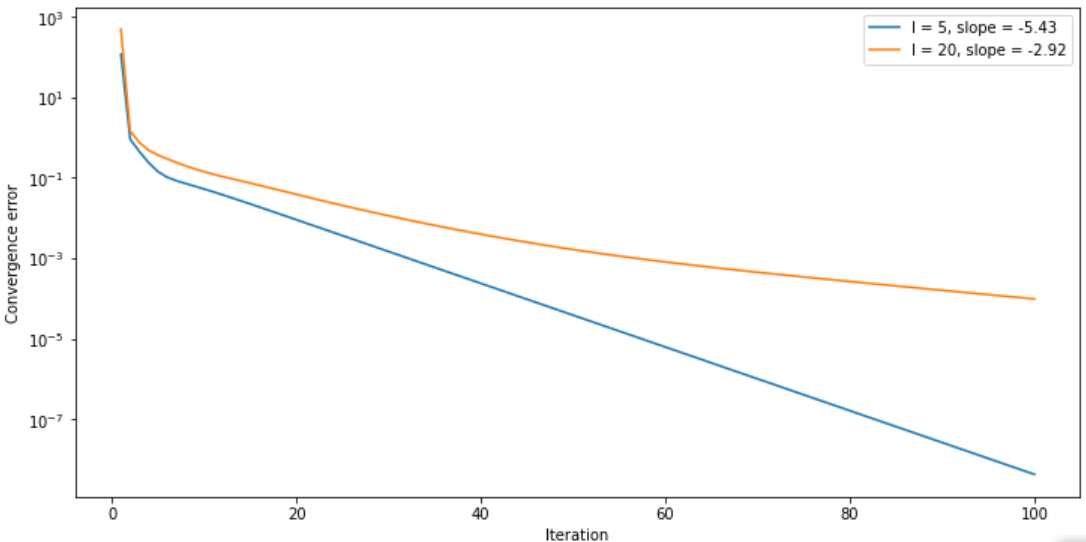
\includegraphics[totalheight=8cm]{convergence.png}
    \caption[]{Convergence of \( V^{(k)} \) to \( V_1 \) as a function of iteration}
    \label{fig:verticalcell}
\end{figure}

\begin{figure}
    \centering
    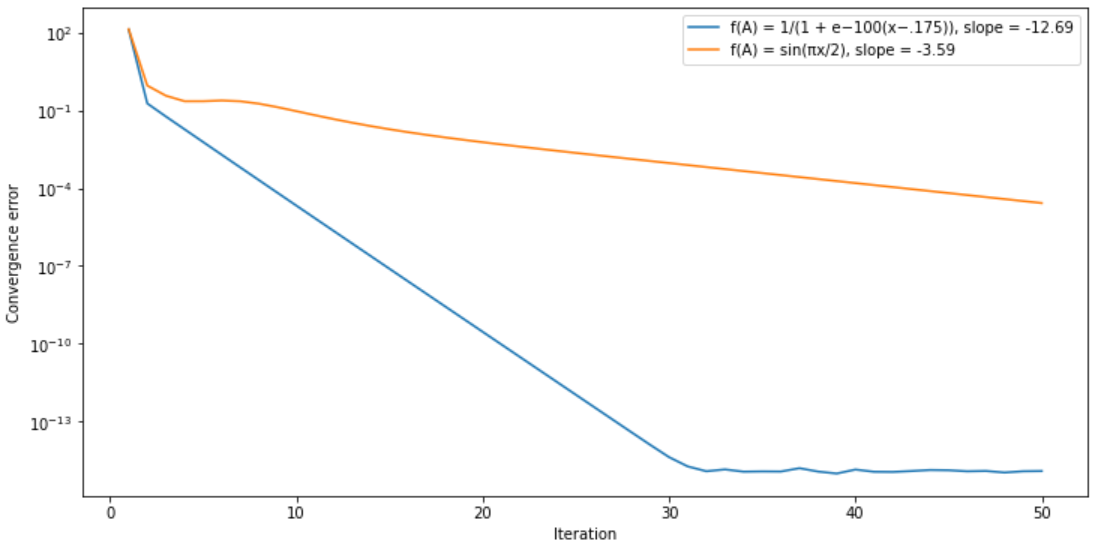
\includegraphics[totalheight=8cm]{func_convergence.png}
    \caption{Convergence of \( V^{(k)} \) to \( V_1 \) as a function of iteration for the two functions}
    \label{fig:verticalcell}
\end{figure}

\begin{enumerate}[label=(\alph*)]
    \item Let $V_1\in\R^{n\times \ell}$ represent the eigenvectors associated with $\lambda_1$ through $\lambda_\ell.$ For $\ell = 5$ and $\ell = 20$ run simultaneous iteration to approximate $V_1$ and plot the convergence of $V^{(k)})$ to $V_1$ as a function of iteration. How do you expect the error to behave and do your results match your expectations? Why or why not? \\
          \textbf{Solution:} Given a symmetric matrix \( A \) of size \( 100 \times 100 \) with eigenvalues \( \lambda_i = \frac{1}{i} \), the convergence of a simultaneous iteration for approximating eigenvectors depends critically on the spectral gap. The spectral gap, defined as the difference between successive eigenvalues \( \lambda_{i} - \lambda_{i+1} \), diminishes as \( i \) increases. Consequently, the convergence is more rapid for smaller indices due to larger gaps. Specifically, when \( \ell = 5 \), the subspace iteration converges more swiftly as it encompasses eigenvalues with larger gaps, implying faster eigenvector approximation.

          As shown in figure 1, the slope of convergence is steeper for \( \ell = 5 \) than for \( \ell = 20 \), indicating faster convergence for the former. This aligns with our expectations, as the spectral gap is larger for smaller indices, leading to faster convergence. The results are consistent with our expectations, demonstrating the influence of the spectral gap on the convergence of simultaneous iteration.

    \item Consider the following two functions:
          \begin{equation*}
              \begin{aligned}
                  (1) \quad f(x) & = \sin(\pi x / 2)         \\
                  (2) \quad f(x) & = 1/(1+e^{-100(x-.175)}).
              \end{aligned}
          \end{equation*}
          For the problem in part (a) with $\ell = 5,$ would running subspace iteration with these functions help us converge to $V_1$ in fewer iterations? Please answer the question for both functions and justify your response. \\
          \textbf{Solution:}
          The convergence of subspace iteration for a transformed matrix \( f(A) \) depends on how the transformation function \( f \) alters the eigenvalues of \( A \). Given the eigenvalue distribution of \( A \) with \( \lambda_i = \frac{1}{i} \), we consider the two suggested functions:

          \begin{equation*}
              \begin{aligned}
                  (1) \quad f(x) & = \sin\left(\frac{\pi x}{2}\right) \\
                  (2) \quad f(x) & = \frac{1}{1+e^{-100(x-0.175)}}.
              \end{aligned}
          \end{equation*}

          For \( \ell = 5 \), function (1) transforms the eigenvalues into a sinusoidal pattern which has the effect of clustering the transformed eigenvalues \( f(\lambda_i) \) closer together, thus reducing the spectral gaps and potentially slowing the convergence for the dominant eigenspace.

          Function (2) is a sigmoid function that sharply increases around \( x = 0.175 \). This transformation will drastically amplify the spectral gap between the eigenvalues less than \( 0.175 \) and those greater than \( 0.175 \). Since \( \lambda_5 = 0.2 \), the spectral gap around \( \lambda_5 \) is significantly increased, likely accelerating the convergence of subspace iteration towards the eigenvectors corresponding to the largest transformed eigenvalues \( f(\lambda_1) \) through \( f(\lambda_5) \).

          Therefore, while function (1) may not facilitate faster convergence, function (2) is expected to enhance the separation between the dominant eigenvalues and the rest, thus aiding in more rapid convergence to \( V_1 \) for \( \ell = 5 \).

          As shown in figure 2, the convergence of subspace iteration for function (2) is significantly faster than both the original and function (1), aligning with our expectations. This demonstrates the influence of the transformation function on the convergence of subspace iteration, with function (2) accelerating the convergence for \( \ell = 5 \).

\end{enumerate}


\subsection*{Question 5 (12 points)}
Consider $A\in\R^{m\times n}$ with $m< n.$
\begin{enumerate}[label=(\alph*)]
    \item Prove that the least squares problem
          \[
              \min_x \|Ax - b\|_2^2
          \]
          has an infinite number of solutions for any $b.$

          \textbf{Solution:} Given a matrix $A \in \mathbb{R}^{m \times n}$ with $m < n$, we aim to demonstrate that the least squares problem $\min_x \|Ax - b\|_2^2$ has an infinite number of solutions for any $b$.

          \textbf{Proof:}

          \begin{enumerate}
              \item \textbf{Rank and Dimensions:}

                    Since $A$ has more columns than rows ($m < n$), it follows that $\text{rank}(A) \leq m$. This implies that $A$ cannot span $\mathbb{R}^n$, leading to a non-trivial null space $\mathcal{N}(A)$, meaning there exists at least one non-zero vector $v \in \mathbb{R}^n$ such that $Av = 0$.

              \item \textbf{Infinite Solutions:}

                    For any solution $x$ to the least squares problem, we can add any vector $v \in \mathcal{N}(A)$ to $x$ without affecting the residual norm $\|Ax - b\|_2^2$. This is because $A(x + v) = Ax + Av = Ax$, and the residual norm remains the same.
          \end{enumerate}

          \textbf{Conclusion:}

          Thus, the least squares problem $\min_x \|Ax - b\|_2^2$ admits an infinite number of solutions for any $b$ when $A \in \mathbb{R}^{m \times n}$ with $m < n$, due to the underdetermined nature of the system and the existence of a non-trivial null space for $A$.

    \item Prove that for any non-singular $M\in\Rn$ the regularized problem
          \begin{equation}
              \label{eqn:LS}
              \min_x \|Ax - b\|_2^2 + \|Mx\|_2^2
          \end{equation}
          has a unique solution.

          \textbf{Solution:} Given the regularized problem:
          \[
              \min_x \|Ax - b\|_2^2 + \|Mx\|_2^2,
          \]
          the objective function is:
          \[
              f(x) = (Ax - b)^T(Ax - b) + (Mx)^T(Mx).
          \]

          \textbf{First Derivative (Gradient):}
          Taking the gradient of $f(x)$ with respect to $x$, we obtain:
          \[
              \nabla f(x) = 2A^T(Ax - b) + 2M^TMx.
          \]

          \textbf{Second Derivative (Hessian):}
          The Hessian $H$ of $f(x)$ is:
          \[
              H = \nabla^2 f(x) = 2A^TA + 2M^TM.
          \]

          \textbf{Strict Convexity:}
          The function $f(x)$ is strictly convex if its Hessian is positive definite. Since $A^TA$ is positive semi-definite and $M^TM$ is positive definite (as $M$ is non-singular), the sum $A^TA + M^TM$ is positive definite.

          Horn, Roger A.; Johnson, Charles R. (2013). Matrix Analysis (2nd ed.).

          \[
              x^T(A^TA + M^TM)x = x^TA^TAx + x^TM^TMx > 0, \quad \forall x \neq 0.
          \]
          because $x^TM^T M x > 0$ for $x \neq 0$ and $x^T A^T A x \geq 0$ for all $x$.

          Therefore, $f(x)$ is strictly convex.

          \textbf{Conclusion:}
          Therefore, the objective function $f(x)$ is strictly convex, ensuring the uniqueness of the global minimum. Hence, the given regularized problem has a unique solution.

    \item Provide an algorithm that solves~\eqref{eqn:LS} in $\cO(n^3)$ time. Be sure to show why your algorithm returns the desired result. \\
          \textbf{Solution:}
          To solve the regularized least squares problem
          \[
              \min_x \|Ax - b\|_2^2 + \|Mx\|_2^2,
          \]
          we derive an explicit solution and propose an algorithm with computational complexity $\mathcal{O}(n^3)$.
          \textbf{First Derivative (Gradient):}
          Taking the gradient of $f(x)$ with respect to $x$, we obtain:
          \[
              \nabla f(x) = 2A^T(Ax - b) + 2M^TMx.
          \]

          We can equate the gradient to zero to obtain the solution:
          Therefore,

          \begin{align*}
              2A^T(A\hat{x} - b) + 2M^TM\hat{x} & = 0     \\
              A^TA\hat{x} + M^TM\hat{x}         & = A^Tb.
          \end{align*}


          The solution is given by the linear system:
          \[
              (A^TA + M^TM)\hat{x} = A^Tb.
          \]

          \textbf{Algorithm:}
          \begin{enumerate}
              \item Compute $A^TA$ and $M^TM$. It takes $\mathcal{O}(mn^2)$ and $\mathcal{O}(n^3)$ time, respectively.
              \item Sum $A^TA$ and $M^TM$ to form $(A^TA + M^TM)$. It takes $\mathcal{O}(n^2)$ time.
              \item Use the Cholesky factorization to compute the $LU$ decomposition of $(A^TA + M^TM)$. It takes $\mathcal{O}(n^3)$ time.
              \item Solve the linear system $(A^TA + M^TM)\hat{x} = A^Tb$ using the $LU$ decomposition. It takes $\mathcal{O}(n^2)$ time using forward and backward substitution.
          \end{enumerate}

          \textbf{Complexity Analysis:}
          The computational complexity is dominated by matrix multiplication and $LU$ decomposition, both of which have a complexity of $\mathcal{O}(n^3)$. The overall complexity of the algorithm is $\mathcal{O}(n^3)$.

          \textbf{Conclusion:}
          This algorithm efficiently computes the unique solution to the regularized least squares problem using standard linear algebra operations.


    \item If $M$ is upper triangular can we solve~\eqref{eqn:LS} asymptotically faster than $\cO(n^3)$? If we can, provide an algorithm to do so, prove its complexity, and show why it returns the desired result.
          \textbf{Solution:}
          The goal is to minimize the regularized least squares objective given by
          \[ \min_{x} \left\| Ax - b \right\|_2^2 + \left\| Mx \right\|_2^2. \]

          Given that \( M \) is a non-singular upper triangular matrix, its singular value decomposition (SVD) has some nice properties. Let the SVD of \( M \) be \( M = XYZ \), where \( X \) and \( Z \) are orthogonal matrices, and \( Y \) is a diagonal matrix whose diagonal values are the singular values of \( M \), which also coincide with the diagonal entries of \( M \) since \( M \) is upper triangular.

          http://arxiv.org/pdf/1202.1490.pdf


          If the SVD of \( A \) is \( A = UEV^T \), where \( U \) and \( V \) are orthogonal, and \( E \) is diagonal, then we can reformulate the normal equation for the regularized problem as

          \[ (A^TA + M^TM)x = A^Tb \]

          which can be written as

          \[ (V E^2 V^T + Y^T Y)^{-1} V E U^T b. \]

          We can note that \( Y^T Y = V Y^T Y V^T \) because \( V \) is an orthogonal matrix and the multiplication by \( V \) and \( V^T \) on either side does not change the diagonal structure of \( Y^T Y \). Therefore, the solution for \( x \) can be expressed as

          \[ x = \left( V(E^2 + Y^T Y)V^T \right)^{-1} VEU^Tb, \]

          which simplifies to

          \[ x = V(E^2 + Y^T Y)^{-1} E U^T b. \]

          The matrix \( E^2 + Y^T Y \) is diagonal, and its inversion can be done efficiently. Let \( E^+ \) be the matrix such that \( E^+_{ii} = \sigma_i / (\sigma_i^2 + M_{ii}^2) \), which represents the updated singular values considering the regularization term. This can be computed in \( \mathcal{O}(n) \) time.

          The dominant computational factor is the SVD of \( A \), which can be computed in \( \mathcal{O}(m^2n) \) time. The matrix multiplications involving orthogonal matrices and diagonal matrices can be done efficiently, and hence, the total computational complexity is dominated by the SVD computation.


          \begin{align*}
              x & = V(E^2 + Y^T Y)^{-1} E U^T b                                                              \\
                & = V \left(\text{diag}\left(\frac{\sigma_i}{\sigma_i^2 + M_{ii}^2}\right)\right)^{-1} U^T b
          \end{align*}

          which provides the solution \( x \) for the regularized least squares problem.




\end{enumerate}
\end{document}